\documentclass[11pt]{article}

\usepackage[T1]{fontenc}
\usepackage{lmodern}
\usepackage{amsmath,amssymb,amsthm}
\usepackage{microtype}
\usepackage{geometry}
\usepackage{xcolor}
\usepackage{graphicx}
\usepackage{hyperref}
\usepackage{enumitem}
\usepackage{booktabs}
\usepackage{tabularx}
\usepackage{listings}
\usepackage{titlesec}
\usepackage{eso-pic}
\usepackage{tikz}
\usetikzlibrary{arrows.meta,positioning,calc,fit}
\geometry{margin=1in}

\definecolor{AIONBlue}{RGB}{20, 60, 120}
\definecolor{AIONAccent}{RGB}{120, 20, 120}
\hypersetup{
    colorlinks=true,
    linkcolor=AIONBlue,
    citecolor=AIONBlue,
    urlcolor=AIONAccent,
    hypertexnames=false
}
\titleformat{\section}{\large\bfseries\color{AIONBlue!85!black}}{\thesection}{0.5em}{}
\titleformat{\subsection}{\normalsize\bfseries\color{AIONBlue!85!black}}{\thesubsection}{0.5em}{}

\theoremstyle{definition}
\newtheorem{definition}{Definition}[section]
\theoremstyle{plain}
\newtheorem{theorem}[definition]{Theorem}
\newtheorem{proposition}[definition]{Proposition}
\newtheorem{corollary}[definition]{Corollary}
\theoremstyle{remark}
\newtheorem{remark}[definition]{Remark}

\newcommand{\WARP}{\textsc{warp}}
\newcommand{\AION}{AI$\Omega$N}
\newenvironment{argument}{\begin{proof}[Argument]}{\end{proof}}

\lstdefinestyle{aionrust}{
  basicstyle=\ttfamily\small,
  frame=single,
  columns=fullflexible,
  keepspaces=true,
  showstringspaces=false,
  breaklines=true
}

\tikzset{
  warpbox/.style={draw, rounded corners=2pt, thick, align=center, minimum height=8mm, inner sep=4pt},
  warpsmall/.style={draw, rounded corners=2pt, align=center, minimum height=6mm, inner sep=3pt},
  warparrow/.style={-Latex, thick},
  warpblocked/.style={-Latex, thick, dashed},
  warplabel/.style={font=\footnotesize},
  warpghost/.style={draw, dashed, rounded corners=2pt, align=center, inner sep=3pt},
  hostnode/.style={circle, draw=black, line width=0.8pt, minimum size=7mm, inner sep=0pt},
  hostedge/.style={-, draw=black, line width=0.8pt},
  matchboxA/.style={draw=black, dashed, rounded corners=2pt, line width=0.8pt, inner sep=4pt},
  matchboxB/.style={draw=black, densely dotted, rounded corners=2pt, line width=0.8pt, inner sep=4pt}
}

\newcommand{\AIONDraftWatermark}{%
  \AddToShipoutPictureBG{%
    \AtPageCenter{%
      \makebox(0,0){%
        \rotatebox{63}{%
          \textcolor{red!14}{\fontsize{68}{74}\selectfont\bfseries ROUGH DRAFT}%
        }%
      }%
    }%
    \AtPageLowerLeft{%
      \raisebox{0.18\paperheight}[0pt][0pt]{%
        \hspace*{0.16in}%
        \rotatebox{90}{%
          \textcolor{AIONAccent!35}{\fontsize{18}{22}\selectfont\bfseries ROUGH DRAFT \quad ROUGH DRAFT \quad ROUGH DRAFT}%
        }%
      }%
    }%
  }%
}

\title{WARP: Recursive Witnessed Admission over Shared Causal History}
\author{James Ross}
\date{Draft 0.1 \\ April 2026}

\begin{document}

\AIONDraftWatermark

\maketitle

\begin{abstract}
We define \WARP{} as a system for admitting claims into shared causal reality, recording why those admissions were lawful, and revealing the resulting history under bounded rights. We argue that the familiar \WARP{} mechanisms---deterministic ticks, provenance-rich worldlines, replayable history, and lawful branching over shared prefixes---are all instances of that deeper invariant. Formally, \WARP{} is a recursive, witnessed admission architecture over bounded frontier-relative causal sites. At each scale, the system takes a plural family of claims, normalises them to a comparable frontier, evaluates them under a governing policy, emits an outcome, and preserves a witness explaining why that outcome is lawful. This admission pattern recurs in local graph rewriting, braid-local collapse over speculative lanes, and distributed suffix reconciliation across replicas: each scale slices claims to a comparable frontier, admits over the bounded site, and packs the witnessed result into an admission hologram. It also clarifies the post-Unix horizon: processes, files, and world states are not ontic containers but frontier-relative materialisations over a shared causal substrate. From that vantage, privacy and provenance are not opposites. The same architecture that commits truth can also fold history and reveal it under law through bounded apertures, author-only speculative lanes, and certificate-bearing collaboration.
\end{abstract}

\section{Introduction}

The preceding \AION{} papers established the pieces that make \WARP{} technically unusual: deterministic execution, provenance-complete boundary artefacts, observer-relative revelation, and executable branching over admissible histories. What remained less explicit was the architectural centre tying those pieces together. The result was a stack that was individually strong but still readily described as a cluster of adjacent mechanisms rather than as one architectural law.

This matters because the distinction at issue is not cosmetic. A system organised around storage, merge, or process isolation makes different promises from a system organised around lawful admission. In the former, history is often an implementation detail and disagreement is pressure toward flattening. In the latter, history is primary, and the system must decide what may become part of shared causal reality, what may remain plural, what must be blocked, and why. That difference is what turns \WARP{} from a collection of mechanisms into a coherent ontology.

The claim of Paper VII is that the architectural centre is not a storage technique, a debugger facility, or a merge strategy. It is an admission law. A \WARP{} system repeatedly decides what may become part of shared causal reality under a policy, over a bounded site, with an explicit witness. This is true when the object under judgement is a local rewrite, when it is a braid of speculative lane claims, and when it is a transported suffix from another replica. Later in the stack, the same logic reappears in softer but no less important forms: deciding what certificates others may rely on, what historical segments may be folded to opaque boundary form, and what an observer may lawfully reveal.

This shift changes what the architecture is \emph{about}. \WARP{} is not simply a graph database with provenance. It is a runtime for committing, folding, and revealing truth under law. Once we state the architecture in those terms, several results that previously appeared separate begin to align. Braids are no longer treated as ordinary merges; they are plural claim objects awaiting admission. ReaderHeads are no longer query interfaces alone; they are revelation surfaces constrained by the ontology of admitted results. Continuum is no longer ``an operating system built on a graph''; it is the operating-system-scale limit of frontier-relative computing.

The newer ontology hidden inside that shift should be stated plainly. There is
no privileged materialised graph sitting underneath the system. What is primary
is witnessed causal history: admitted transitions, frontiers, receipts,
boundary artefacts, and the evidence needed to replay or verify them. When we
still speak of ``the graph,'' we mean a coordinate chart over that history: an
observer-relative holographic reading emitted through a lawful aperture,
basis, and reading discipline. This preserves the utility of graph language
without pretending that a graph-in-itself owns truth. \WARP{} is therefore
graph-expressive without being graph-fundamental.

A brief concrete sketch makes the recurrence clear. At tick scale, suppose two candidate rewrites both touch the same semantic site: one may be admitted, the other blocked, and the witness records why they could not lawfully coexist. At replica scale, suppose a remote suffix arrives from another node: before it can be judged at all, it must be transported to a shared basis, after which admission determines whether the import is lawful, conflicting, plural, or obstructed. The same control shape governs both cases. That recurrence is the central claim of the paper.

\paragraph{Minimal prior knowledge.}
A reader requires only three facts from the earlier papers to follow this one: \WARP{} executes deterministic ticks over bounded sites, preserves provenance-complete boundary artefacts for replay and audit, and supports branching over shared causal history. Paper VII names the architectural law that makes those pieces instances of one system rather than adjacent techniques.

\paragraph{Thesis.}
The thesis sentence we will use throughout is the following:

\begin{quote}
\WARP{} is a recursive, witnessed admission architecture over bounded frontier-relative causal sites.
\end{quote}

The phrase is meant to pay its debts. The causal part descends from the distributed-systems and concurrency insight that event order is fundamentally partial rather than globally sequential \cite{lamport1978time,winskel1986event}. The bounded-site part inherits the locality discipline of algebraic graph transformation and DPO-style rewriting \cite{ehrig1973graph,corradini1997algebraic}. The witness and shell distinction is downstream of provenance work that separates a result from the explanation of why it exists or may be relied upon \cite{buneman2001why,green2007provenance,cheney2009provenance}. What is new here is not any one ingredient, but the claim that the same witnessed admission law recurs at tick, braid, and replica scale.

\paragraph{Position in the series and neighbouring work.}
This paper does not replace the earlier foundations papers; it extracts the invariant they had already approached in part. The present discussion therefore sits at the intersection of deterministic rewriting, provenance systems, version and patch theory, replicated data types, and observer-relative debugging. Against graph rewriting, \WARP{} asks not only whether a local rewrite exists, but what witnessed admission makes it lawful. Against patch and version-control systems, it treats a braid as a plural claim object rather than a hidden merge target \cite{jacobson2009darcs,mimram2013patch}. Against CRDTs and Dynamo-style replicated stores, it treats plurality, conflict, and obstruction as lawful first-class outcomes rather than merely as convergence or reconciliation failures \cite{decandia2007dynamo,shapiro2011crdt}. Against event sourcing, it agrees that present state is derived from history, but makes admission law, witness structure, and bounded revelation native architectural objects \cite{fowler2005eventsourcing}.

\paragraph{Contributions.}
The specific contributions are:

\begin{enumerate}[leftmargin=*]
  \item A generic admission kernel, \(\operatorname{Admit}_{\Pi}(F_*, C, \chi) = (R, W)\), together with a separate packaging act \(\operatorname{Pack}(R, W) = \theta\), making explicit the distinction between witness and shell.

  \item A scale-by-scale identification of the same admission pattern in three primary settings: local tick admission, braid-local admission, and distributed suffix admission after transport to a common basis.

  \item A three-way architectural decomposition into commitment, folding, and revelation, separating what is true from how it is stored and who may lawfully inspect it.

  \item A post-Unix reframing in which processes and files are treated as materialised views over shared causal history, together with a three-tier ``thinking room'' for socially viable speculative work.

  \item An architectural bridge from provenance to privacy through property certificates, reliance status, and observer rights, showing how bounded revelation can coexist with replayable history.
\end{enumerate}

\paragraph{Structure of the paper.}
Section~2 introduces the noun map required by the rest of the paper: causal lanes, worldlines, strands, and braids. Section~3 defines the generic admission kernel and the commitment/folding/revelation split. Section~4 studies the three primary instantiations at tick, braid, and replica scale. Section~5 gives short worked examples with diagrams. Section~6 turns to the post-Unix horizon and the three-tier thinking room. Section~7 develops the privacy, provenance, and revelation layer. Section~8 records the principal open frontier questions, and Section~9 concludes.

\paragraph{Scope.}
This paper is architectural rather than fully formal. Its goal is to extract the common control shape that recurs across the \WARP{} stack and to show how that shape supports both strong provenance and bounded revelation. We therefore do not attempt to finish every frontier law opened by this view. In particular, contamination calculus, collective sovereignty, and export semantics remain follow-on work. The present paper instead fixes the architectural centre with sufficient precision that those later laws can be treated as extensions rather than as hidden prerequisites.

\clearpage

\section{Causal Lanes, Strands, and Braids}

Before stating the admission kernel, we need the basic ontology. The earlier papers developed deterministic execution, branching, and replay, but they did not need to stabilise the noun map at this level of explicitness. Paper VII does, because the same admission law is going to act over different kinds of objects, and those objects must not be allowed to collapse into one another.

\begin{definition}[Causal lane]
A \emph{causal lane} is a replayable carrier of causal history equipped with a frontier-relative materialisation map. At minimum, a lane has:
\begin{enumerate}[leftmargin=*]
  \item an identity,
  \item an event order or tick order,
  \item a causal provenance record,
  \item and a rule by which a frontier or tick determines a materialised state.
\end{enumerate}
\end{definition}

This use of lanes is intentionally close to the older language of events, causal dependence, and partial orders: it assumes that a computation is not adequately described by one privileged serial timeline \cite{lamport1978time,winskel1986event}.

The term \emph{lane} is therefore the ontology-level noun for a history-bearing computational object. It is intentionally broader than \emph{worldline}. A lane may be canonical or speculative; it may already be socially admitted, or it may still be a private counterfactual carrier.

\begin{definition}[Worldline]
A \emph{worldline} is a canonically admitted causal lane. It is the lane form whose history and frontier-relative materialisations count as shared causal reality for the relevant policy frame.
\end{definition}

\begin{definition}[Strand]
A \emph{strand} is a speculative causal lane rooted at a parent worldline and a fork anchor. A strand carries fork provenance back to that parent anchor, together with whatever local history is required for the strand to diverge lawfully from the inherited base.
\end{definition}

Two consequences should be kept explicit. First, a strand is still a real lane rather than a temporary UI fiction. Secondly, a strand is not defined by being a frozen snapshot. Its materialisation at a given frontier is obtained by resolving the strand's local divergence against the inherited parent history at the chosen basis.

Operationally, this means a strand should be understood holographically rather
than as a fully copied child world. A bounded read of a strand need only
materialise the backward causal cone required by the strand's local divergence
and optic footprint at the chosen basis. The strand is real as a speculative
lane; its realised state remains a frontier-relative reading over inherited
history plus local divergence, not a requirement to eagerly copy the whole
parent lane.

\begin{definition}[Braid]
A \emph{braid} is a plural composition over a family of lanes sharing a common precursor or comparison basis. A braid is not itself a lane. It is a structured plural object that presents multiple validated lane claims over a common frontier so that a later collapse or admission act may judge them.
\end{definition}

This is the first place where ordinary version-control language becomes misleading. A braid is not a latent merge result. It is the plural object over which collapse may later derive a lane-level result, preserve plurality, surface conflict, or return obstruction. The name nods to the geometric intuition of intertwined strands, but the paper does not rely on braid-group algebra; the load-bearing ancestry is patch theory, concurrency semantics, and witnessed admission.

\begin{remark}[Ontology versus realisation]
The nouns above are ontology-level nouns. Realisation-level objects are frontier-relative views: a strand resolved at a particular parent frontier, or a braid presented over a specific common basis. This distinction is necessary because a strand may be a stable noun while its realised view changes with the frontier at which it is interpreted.
\end{remark}

The same split also prevents admission from silently doing other jobs. Forking creates ancestry. Braiding constructs a plural comparison object. Collapse derives a lane-level result from that plural object when policy and witness conditions allow it. Admission, finally, blesses a derived result as canonical when the governing law requires that further step. If these verbs are allowed to blur together, the rest of the paper becomes incoherent.

\paragraph{Operational intuition.}
A worldline is the shared lane others may rely on. A strand is the speculative lane in which counterfactual or author-local work may proceed without immediately becoming shared fact. A braid is the object that appears when several such lanes must be compared over one basis without yet pretending they have collapsed into a single answer. The admission kernel introduced next acts over all three scales, but it acts over different objects at each scale.

\paragraph{Specification note.}
The paper deliberately keeps the runtime interface out of line. The noun map above is implementation-bearing, but code signatures belong in the companion runtime RFC, where trait bounds, retention posture, authority context, and witness carriers can be checked rather than merely gestured at. Here the useful artefact is the invariant control shape, not a language binding.

\section{The Generic Admission Kernel}

The first distinction to keep clean is that the plural claim object is not the admission act. At any scale, the system begins with:

\begin{itemize}[leftmargin=*]
  \item a normalised frontier-relative base \(F_*\),
  \item a plural family of claims \(C\),
  \item a bounded site or refined site family \(\chi\),
  \item a governing law or policy \(\Pi\),
  \item and witness-bearing local geometry describing why an outcome is lawful.
\end{itemize}

\begin{definition}[Admission slice]
The bounded site \(\chi\) is the \emph{admission slice}: the least frontier-relative closure over which the governing policy can lawfully compare the plural claims and judge their coexistence, derivation, plurality, conflict, or obstruction. The normaliser produces claims over such a slice; the shell later preserves the result slice needed for replay, audit, transport, or revelation. This generalises the spirit of program slicing---isolating what is relevant to a criterion---from program statements to witnessed causal history \cite{weiser1981program}.
\end{definition}

We therefore write the generic admission act as:

\[
\operatorname{Admit}_{\Pi}(F_*, C, \chi) = (R, W)
\]

followed by:

\[
\operatorname{Pack}(R, W) = \theta
\]

where \(R\) is the admitted outcome, \(W\) is the witness core, and \(\theta\) is the shell or receipt-like package used for replay, audit, or transport.

One useful typing makes the outcome space explicit. Let \(X\) be the
scale-local carrier of derived results. Then

\[
\mathcal{O}(X)
:=
X
\;\sqcup\;
\operatorname{Plural}(X)
\;\sqcup\;
\operatorname{Conflict}
\;\sqcup\;
\operatorname{Obstruction}.
\]

Thus the admission act is not Boolean. It returns a witnessed member of an
outcome algebra.

The separation between \(W\) and \(\theta\) is important. The witness is the semantic explanation of lawfulness; in the constructive tradition, it plays the role of a proof-bearing object rather than an after-the-fact annotation \cite{martinlof1984intuitionistic}. The shell is the carrier. A Boundary Transition Record is therefore not the admission law itself; it is the package that anchors the law's result for later use.

\begin{definition}[Admission hologram]
For a policy \(\Pi\), bounded site \(\chi\), and admitted pair \((R, W)\), an
\emph{admission hologram} is a shell
\[
\theta = \operatorname{Pack}(R, W)
\]
together with any referenced basis anchors, such that \(\theta\) is
information-complete for the admitted local situation at that site up to the
equivalence required for replay, audit, transport, or revelation. Its contract
is not to preserve an entire materialised world. Its contract is to preserve
the least lawful boundary from which the admitted outcome and its
witness-bearing consequences can be reconstructed.
\end{definition}

\begin{proposition}[Recursive admission holograms]
For each primary scale
\(s \in \{\mathrm{tick}, \mathrm{braid}, \mathrm{replica}\}\),
the scale-local pipeline
\[
\widehat{C}_s
\xrightarrow{\operatorname{Slice}_s}
(C_s,\chi_s)
\xrightarrow{\operatorname{Admit}_{\Pi_s}}
(R_s,W_s)
\xrightarrow{\operatorname{Pack}}
\theta_s
\]
emits an admission hologram \(\theta_s\) for the admitted situation at that scale.
\end{proposition}

\begin{argument}
At tick scale, the input slice is the local footprint closure; the shell preserves the frontier coordinate, the admitted rewrite result, and the blocked-by witness needed to replay one lawful tick. At braid scale, the input slice is the refined comparison basis for participant claims; the shell preserves the common basis, cell geometry, collapse outcome, and witness explaining whether derivation, plurality, conflict, or obstruction was lawful. At replica scale, the input slice is the imported region after transport to a comparable frontier; the shell preserves the comparable basis, imported suffix claims, import outcome, and transport/import witness. In each case the shell is boundary-complete for the bounded admitted situation without preserving an entire materialised history.
\end{argument}

This matters because it extends computational holography beyond ticks. A local
tick receipt is one admission hologram, but so too is a braid-local collapse
artefact and a transport/import shell for replicated suffixes. The recursive
claim is the point: braid merges and distributed imports are not special
mechanisms that happen to carry metadata; they are the same slice--admit--pack
shape applied at a larger frontier. Once stated that way, three consequences follow. First, plural lane situations can be cached,
transported, and reviewed without flattening them into premature canonical
state. Secondly, replicated runtimes can exchange witness-bearing import
holograms rather than opaque packets or materialized frontier snapshots. Thirdly, bounded
observers can decode only the least lawful slice required for a reading,
because the shell already preserves the local situation to be revealed.

Truth should also be read operationally here. In \WARP{}, ``truth'' is not metaphysical truth. It is what may be lawfully admitted relative to a frontier, a policy, and a witness. That is why admission does not reduce to binary accept or reject: lawful outcomes may also preserve plurality, surface conflict, or return obstruction.

\subsection{Commitment, Folding, Revelation}

The same kernel becomes easier to see once the stack is divided into three moments:

\begin{itemize}[leftmargin=*]
  \item \textbf{Commitment}: plural claims are admitted into frontier-relative truth.
  \item \textbf{Folding}: already-admitted history is re-expressed in a boundary-equivalent form.
  \item \textbf{Revelation}: admitted or folded history is exposed to a bounded observer under an aperture and authority regime.
\end{itemize}

This three-way split is one of the paper's main architectural results. It keeps the system from conflating what is true, how truth is stored, and who may see it.

The equivalence relation below is intentionally behavioural: what matters is not byte identity of shells, but preservation of the lawful observations and replay obligations promised by a retained contract. In that sense it is closer to bisimulation and observational equivalence than to storage equality \cite{park1981concurrency,milner1989communication}.

\begin{definition}[Shell equivalence]
Let \(\Lambda\) be a retained contract specifying which replay, audit,
transport, or revelation obligations must remain lawful. Two shells
\(\theta\) and \(\theta'\) satisfy
\[
\theta \simeq_{\Lambda} \theta'
\]
iff they are both information-complete for the same admitted local situation up
to the lawful uses demanded by \(\Lambda\).
\end{definition}

For later use, the three moments can be written as typed acts:

\[
\operatorname{Commit}_{\Pi}(F_*, C, \chi)
:=
(R, W, \theta)
\]
where
\[
(R, W) = \operatorname{Admit}_{\Pi}(F_*, C, \chi),
\qquad
\theta = \operatorname{Pack}(R, W).
\]

\[
\operatorname{Fold}_{\Lambda}(\theta) = \theta'
\qquad
\text{with}
\qquad
\theta' \simeq_{\Lambda} \theta.
\]

\[
\operatorname{Reveal}_{\Omega,\alpha}(m,\theta)
=
(m', y, W_{\mathrm{rev}})
\]
where \(\Omega = (\pi,\mathcal{B}, M, K, E)\) is an observer plan, \(\alpha\)
is the active authority regime, \(m \in M\) is the current observer state, and
\(y\) is the emitted reading.
This observer plan is the revelation-side object rather than the whole optic:
it fixes what may be projected and emitted, while commitment and witness
preserve the local transformation and reintegration story on which that reading
depends.

\begin{proposition}[Folding preserves lawful readings]
If \(\theta' = \operatorname{Fold}_{\Lambda}(\theta)\) and the retained
contract \(\Lambda\) is sufficient for observer plan \(\Omega\) under authority
regime \(\alpha\), then
\[
\operatorname{Reveal}_{\Omega,\alpha}(m,\theta')
\approx_{\Omega,\alpha}
\operatorname{Reveal}_{\Omega,\alpha}(m,\theta)
\]
where \(\approx_{\Omega,\alpha}\) identifies readings that emit the same lawful
observation at that aperture, basis, and authority tier.
\end{proposition}

\begin{argument}
By shell equivalence, \(\theta\) and \(\theta'\) preserve the same admitted
local situation for the uses demanded by \(\Lambda\). If \(\Lambda\) covers the
observer/authority pair \((\Omega,\alpha)\), then revelation over either shell
has the same lawful reading consequences up to the observer's own reading
equivalence.
\end{argument}

In short: commitment changes what may count as shared truth, folding changes
the carrier while preserving an explicit contract, and revelation changes what
an observer may lawfully emit from that carrier without changing the admitted
situation itself.

\paragraph{Minimal algorithmic form.}
The runtime-facing shape is better stated language-neutrally:
\[
\widehat{C}
\xrightarrow{\text{slice / normalise}}
(C,\chi)
\xrightarrow{\operatorname{Admit}_{\Pi}}
(R,W)
\xrightarrow{\operatorname{Pack}}
\theta .
\]
The point is not a language binding. The point is that the runtime must not collapse the raw claims, comparable slice, admitted result, semantic witness, and shell used for replay or transport into one undifferentiated record.

At this level, policy should remain engine-defined and deterministic, while
hosts select or configure it by reference rather than injecting bespoke
admission code. A local tick may choose a Boundary Transition Record as one
concrete shell family; suffix transport, settlement publication, or bounded
revelation need not reuse that same carrier.

\section{The Primary Triad}

The admission kernel recurs most cleanly in three primary instantiations.

\begin{proposition}[Admission-shape invariance]
For each primary scale
\(s \in \{\mathrm{tick}, \mathrm{braid}, \mathrm{replica}\}\),
there exist typed objects
\((F_s, C_s, \chi_s, \Pi_s)\)
and a scale-local carrier \(X_s\) such that
\[
(R_s, W_s) = \operatorname{Admit}_{\Pi_s}(F_s, C_s, \chi_s),
\qquad
R_s \in \mathcal{O}(X_s).
\]
For replica admission, \(C_s\) exists only after transport has normalised remote
claims to a comparable frontier.
\end{proposition}

\begin{argument}
At tick scale, the claims are candidate local rewrites over one current
frontier. At braid scale, the claims are validated strand-local claims
presented over one common basis. At replica scale, the claims are remote suffix
claims only after transport has mapped them to a comparable frontier. In each
case the same admission signature applies: a frontier-relative base, a plural
claim object, a bounded site, a governing law, and a witnessed outcome.
\end{argument}

\begin{corollary}[Slicing / normalisation law]
Let \(\widehat{C}_s\) denote the raw scale-local claim family before
comparability has been established. Then for each primary scale there exists a
normaliser
\[
\operatorname{Norm}_s(F_s, \widehat{C}_s) = C_s
\]
such that
\[
(R_s, W_s)
=
\operatorname{Admit}_{\Pi_s}
\bigl(F_s, \operatorname{Norm}_s(F_s, \widehat{C}_s), \chi_s\bigr).
\]
At tick scale, \(\operatorname{Norm}_{\mathrm{tick}}\) is the identity on
already local candidate rewrites. At braid scale,
\(\operatorname{Norm}_{\mathrm{braid}}\) presents validated strand claims over
a common basis. At replica scale, \(\operatorname{Norm}_{\mathrm{replica}}\)
is transport to a comparable frontier.
\end{corollary}

\begin{argument}
This is the preceding proposition with the comparability step made explicit as a
separate map. The map is a slicer: it rejects the whole-world view and presents only the comparable closure required for admission.
\end{argument}

The practical consequence is that distance does not create a new kind of
resolution problem in \WARP{}. It changes the normalisation required before
admission. Ordinary systems often treat distribution as a separate class of
reconciliation problem because history, basis, and witness are under-specified.
\WARP{} promotes those preconditions into explicit structure and then reuses
the same witnessed admission law. Distribution changes the slice boundary; it
does not change the admission law.

\subsection{Local Tick Admission}

At engine scale, the base frontier is the current state, the plural claim object is the candidate rewrite bundle, the bounded sites are local footprints, and the governing policy is the scheduler or local coexistence law for that tick. Here the bounded site is the admission-side focal closure: the footprint together with enough affected and reintegration structure to judge coexistence lawfully. Admission decides which rewrites may coexist lawfully in one tick and emits both the next state and a witness of blocked and admitted structure. Consider the simplest case: if two candidates both attempt to mutate the same semantic node footprint, one may be admitted while the other is blocked, with the witness preserving exactly why that obstruction occurred.

\[
(R_{\mathrm{tick}}, W_{\mathrm{tick}})
=
\operatorname{Admit}_{\Pi_{\mathrm{sched}}}
(F_{\mathrm{tick}}, C_{\mathrm{rw}}, \chi_{\mathrm{fp}}),
\qquad
R_{\mathrm{tick}} \in \mathcal{O}(X_{\mathrm{rw}}).
\]

The corresponding shell
\(\theta_{\mathrm{tick}} = \operatorname{Pack}(R_{\mathrm{tick}}, W_{\mathrm{tick}})\)
is the tick-local admission hologram. It preserves enough boundary information
to replay the lawful local step and its blocked alternatives without
materialising the whole host history.

\subsection{Braid Admission}

At lane scale, the base frontier is a common parent frontier, the plural claim object is a braid, the bounded sites are the refined braid cells, and the governing policy is the braid-scale collapse law. A braid is a structured superposition of validated strand claims over that common basis. A braid is not collapse. Collapse is the admission act performed over the braid. The lawful result space therefore includes more than successful derivation:

\begin{itemize}[leftmargin=*]
  \item \texttt{Derived},
  \item \texttt{Plural},
  \item \texttt{Conflict},
  \item \texttt{Obstruction}.
\end{itemize}

\[
(R_{\mathrm{braid}}, W_{\mathrm{braid}})
=
\operatorname{Admit}_{\Pi_{\mathrm{collapse}}}
(F_{\mathrm{braid}}, B, \chi_{\mathrm{cell}}),
\qquad
R_{\mathrm{braid}} \in \mathcal{O}(X_{\mathrm{lane}}).
\]

The corresponding shell
\(\theta_{\mathrm{braid}} = \operatorname{Pack}(R_{\mathrm{braid}}, W_{\mathrm{braid}})\)
is a braid-level admission hologram. It preserves the comparison basis, the
plural claim geometry relevant to the bounded cells, the admitted collapse
outcome, and the witness that makes that outcome reviewable or transportable
without forcing premature flattening.

This is one of the paper's most important corrections to ordinary branching language. Irreducible plurality is not a failed merge. It is often the lawful admitted result. This is the sharp contrast with convergence-first CRDT presentations and with editing systems whose central obligation is to transform concurrent operations into a single consistent document state \cite{ellis1989groupware,shapiro2011crdt}.

That departure from ordinary version-control intuition matters. If two strands make incompatible but separately valid claims over the same inherited basis, the system need not pretend that a single answer already exists. It may lawfully preserve the result as plural until later adjudication or further evidence changes the situation.

\subsection{Distributed Suffix Admission}

At replica scale, the base frontier is the common replicated prefix, the plural claim object is the family of transported remote suffix claims, the bounded sites are the affected imported regions, and the governing policy is the local transport-and-import law. This sits downstream of Lamport's causal ordering insight and of the later replicated-state lineage, but relocates the hard work into explicit transport and witnessed import \cite{lamport1978time,decandia2007dynamo,shapiro2011crdt}. Normalization is the hard part. Suffixes must first be transported to a common frontier before the same admission algebra can be applied. This is the architectural bridge to Observer Geometry II: the transport square is the precondition under which claims become comparable, after which admission and observer-relative consequences can be studied cleanly. The important correction is that replicas are not synchronising materialized frontier snapshots. They are exchanging witnessed causal suffixes and then admitting those suffixes relative to local frontier truth. Replica distance therefore changes the required normaliser, not the underlying admission signature.

\[
\widetilde{C}_{\mathrm{rep}}
:=
\operatorname{Transport}(F_{\mathrm{rep}}, \Sigma_{\mathrm{remote}}, F_{\mathrm{recv}})
\]
\[
(R_{\mathrm{rep}}, W_{\mathrm{rep}})
=
\operatorname{Admit}_{\Pi_{\mathrm{import}}}
(F_{\mathrm{rep}}, \widetilde{C}_{\mathrm{rep}}, \chi_{\mathrm{imp}}),
\qquad
R_{\mathrm{rep}} \in \mathcal{O}(X_{\mathrm{imp}}).
\]

The corresponding shell
\(\theta_{\mathrm{rep}} = \operatorname{Pack}(R_{\mathrm{rep}}, W_{\mathrm{rep}})\)
is a transport/import hologram. It preserves the comparable basis established
by transport, the import judgement, and the witness needed for replayable
catch-up, audited settlement, or bounded revelation at the receiving runtime.

\begin{theorem}[Independent suffix confluence up to shell equivalence]
Let \(\widehat{C}_1\) and \(\widehat{C}_2\) be two remote suffix claim
families. Let
\[
\widetilde{C}_i
:=
\operatorname{Norm}_{\mathrm{replica}}(F_{\mathrm{rep}}, \widehat{C}_i)
\]
be their transports to a common comparable frontier \(F_{\mathrm{rep}}\). Let
\(\chi_{12}\) be the common site refinement induced by the imported region, and
let \(\chi_1,\chi_2\) be its projections to the individually imported sites.
Assume:

\begin{enumerate}[leftmargin=*]
  \item there exist individual commitments
  \[
  (R_i, W_i, \theta_i)
  :=
  \operatorname{Commit}_{\Pi_{\mathrm{import}}}
  (F_{\mathrm{rep}}, \widetilde{C}_i, \chi_i)
  \]
  with derived outcomes \(R_i \in X_{\mathrm{imp}}\), and let \(F_i\) be the
  derived frontier exposed by \(\theta_i\);

  \item the re-normalised follow-on families
  \[
  \widetilde{C}_2^{(1)}
  :=
  \operatorname{Norm}_{\mathrm{replica}}(F_1, \widehat{C}_2),
  \qquad
  \widetilde{C}_1^{(2)}
  :=
  \operatorname{Norm}_{\mathrm{replica}}(F_2, \widehat{C}_1)
  \]
  remain lawful for import over refined sites
  \(\chi_2^{(1)}\) and \(\chi_1^{(2)}\);

  \item witness-preserving independence holds: admitting either transported
  family preserves, up to shell equivalence, the basis, site refinement, and
  witness conditions required to admit the other.
\end{enumerate}

Write
\[
(R_{12}, W_{12}, \theta_{12})
:=
\operatorname{Commit}_{\Pi_{\mathrm{import}}}
(F_{\mathrm{rep}}, \widetilde{C}_1 \sqcup \widetilde{C}_2, \chi_{12})
\]
for one-shot combined import. Write
\[
(R_{1;2}, W_{1;2}, \vartheta_{1;2})
:=
\operatorname{Commit}_{\Pi_{\mathrm{import}}}
(F_1, \widetilde{C}_2^{(1)}, \chi_2^{(1)})
\]
and
\[
(R_{2;1}, W_{2;1}, \vartheta_{2;1})
:=
\operatorname{Commit}_{\Pi_{\mathrm{import}}}
(F_2, \widetilde{C}_1^{(2)}, \chi_1^{(2)}).
\]
Let \(\Theta_{1;2}\) and \(\Theta_{2;1}\) denote the \(\Lambda\)-retained shells
for the two-step paths \((\theta_1, \vartheta_{1;2})\) and
\((\theta_2, \vartheta_{2;1})\), respectively. Then for any retained contract
\(\Lambda\) covering replay and audit of the imported region,
\[
\theta_{12}
\simeq_{\Lambda}
\Theta_{1;2}
\simeq_{\Lambda}
\Theta_{2;1}.
\]
\end{theorem}

\begin{proof}
The individual commitments provide the two frontier advances \(F_1\) and \(F_2\).
Witness-preserving independence ensures that re-normalising the second suffix
against either derived frontier yields a lawful follow-on import without losing
the basis, site, or witness information required by the retained contract
\(\Lambda\). The one-shot import shell \(\theta_{12}\) and the two sequential
path shells \(\Theta_{1;2}\) and \(\Theta_{2;1}\) therefore preserve the same
admitted local situation, replay obligations, and audited consequences for the
imported region. Hence they are shell-equivalent under \(\Lambda\), even though
the runtime may have reached them by different admissible paths.
\end{proof}

\begin{corollary}[Non-independent suffixes]
If the transported suffix families are not independent, Paper VII does not
assert commutativity or confluence. The receiving runtime still evaluates the
bounded imported site under the same admission kernel and returns a witnessed
member of the outcome algebra
\(\mathcal{O}(X_{\mathrm{imp}})\): derived result, preserved plurality,
conflict, or obstruction.
\end{corollary}

This also identifies the safe availability zone more precisely than ordinary
replication slogans do. The easy distributed case is not ``the whole AP
system.'' It is the footprint-independent fragment of the workload: imported
claim families whose bounded sites can be transported and admitted without
destroying one another's witness conditions.

That is why the theorem above targets shell equivalence rather than naive final
state agreement. Two import paths may agree on a terminal frontier while still
differing in retained witness, replay obligations, or intent preservation. The
architecturally relevant invariant is therefore stronger than state equality
alone.

One immediate consequence is that replication state becomes more than a log of packets or eventual values. If remote suffixes are represented as witnessed transport objects, then a replicated system becomes queryable as a temporal causal structure rather than merely debuggable after the fact. In particular, one should expect a CTL*-like family of queries over lawful transport and admission paths: not only what a replica currently believes, but what imports were possible, what conflicts were inevitable, what acknowledgements must eventually arise under policy, and what an observer at a bounded aperture was entitled to see or rely on along a branch. We do not formalise that logic here, but we do identify the prerequisite: replication must first be promoted into witnessed causal structure.

\section{Illustrative Examples}

The preceding triad is easier to retain when each case is grounded in one concrete example. We therefore record three minimal worked examples, one for each primary scale.

\subsection{Example 1: Local Overlap In One Tick}

Let the current frontier \(F_*\) materialize a local reading containing a node \(n\) with status \texttt{draft}. Suppose the candidate bundle \(C = \{c_1, c_2\}\) contains two local rewrites: \(c_1\) changes \(n\) to \texttt{published}, while \(c_2\) changes the same node to \texttt{archived}. The bounded site \(\chi\) is the semantic footprint containing \(n\) together with whatever neighbourhood is required for the scheduler to judge the update lawfully. The governing policy \(\Pi\) requires exclusive mutation over that footprint within a single tick.

\begin{center}
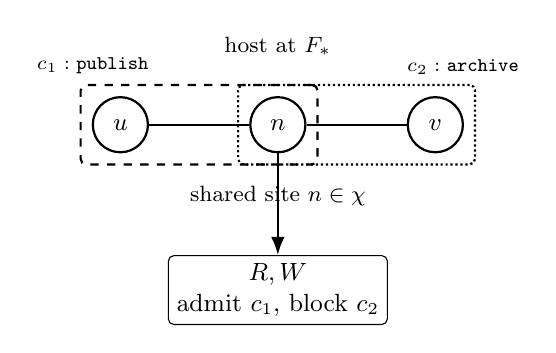
\begin{tikzpicture}[every node/.style={font=\small}]
  \node[hostnode] (u) at (0,0) {$u$};
  \node[hostnode] (n) at (2,0) {$n$};
  \node[hostnode] (v) at (4,0) {$v$};

  \draw[hostedge] (u) -- (n);
  \draw[hostedge] (n) -- (v);

  \node[matchboxA, fit=(u)(n), label={[font=\scriptsize]above left:$c_1:\texttt{publish}$}] {};
  \node[matchboxB, fit=(n)(v), label={[font=\scriptsize]above right:$c_2:\texttt{archive}$}] {};

  \node[warplabel] at (2,1.0) {host at \(F_*\)};
  \node[warplabel] at (2,-0.9) {shared site \(n \in \chi\)};
  \node[warpsmall] (res) at (2,-2.1) {\(R,W\)\\admit \(c_1\), block \(c_2\)};

  \draw[warparrow] (n.south) -- (res.north);
\end{tikzpicture}

\smallskip
\emph{Figure 1.} DPO-style overlapping matches over a shared host site \cite{ehrig1973graph,corradini1997algebraic}. The two candidates overlap on \(n\), so admission preserves the admitted rewrite together with a witness of the blocked alternative.
\end{center}

In this case admission cannot lawfully admit both candidates. A typical result is that one candidate is admitted, the other is blocked, and the witness \(W\) records that the candidates overlapped on the same semantic site under an exclusivity policy. The engineering implication is straightforward: the receipt is not merely a log of what happened, but a replayable explanation of why the blocked candidate could not lawfully coexist in that tick.

\[
(R, W)
=
\operatorname{Admit}_{\Pi}(F_*, \{c_1, c_2\}, \chi),
\qquad
R \in \{\operatorname{Derived}(c_1), \operatorname{Derived}(c_2)\}.
\]

\subsection{Example 2: A Braid That Remains Plural}

Let two strands \(S_1\) and \(S_2\) share a common parent frontier \(F_*\). Each strand carries a valid claim over the same inherited object, but the claims are incompatible: \(S_1\) records one lawful update to the object, while \(S_2\) records another lawful update that cannot be jointly derived under the braid collapse policy \(\Pi\). The refined braid cells \(\chi\) isolate the shared site together with the local reintegration seams needed for comparison.

\begin{center}
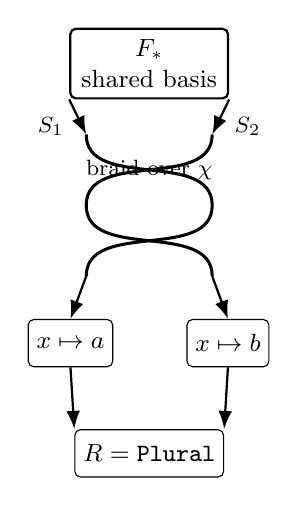
\begin{tikzpicture}[every node/.style={font=\small}]
  \node[warpbox] (base) at (2,3.2) {\(F_*\)\\shared basis};
  \coordinate (l0) at (1.2,2.3);
  \coordinate (r0) at (2.8,2.3);
  \coordinate (l1) at (2.8,1.4);
  \coordinate (r1) at (1.2,1.4);
  \coordinate (l2) at (1.2,0.5);
  \coordinate (r2) at (2.8,0.5);
  \node[warplabel] at (0.75,2.4) {\(S_1\)};
  \node[warplabel] at (3.25,2.4) {\(S_2\)};
  \node[warplabel] at (2,1.85) {braid over \(\chi\)};
  \node[warpsmall] (claima) at (1.0,-0.35) {\(x \mapsto a\)};
  \node[warpsmall] (claimb) at (3.0,-0.35) {\(x \mapsto b\)};
  \node[warpsmall] (plural) at (2,-1.75) {\(R = \texttt{Plural}\)};

  \draw[warparrow] (base.south west) -- (l0);
  \draw[warparrow] (base.south east) -- (r0);

  \draw[line width=1.1pt] (l0) to[out=-90,in=90] (l1) to[out=-90,in=90] (l2);
  \draw[line width=1.1pt] (r0) to[out=-90,in=90] (r1) to[out=-90,in=90] (r2);

  \draw[warparrow] (l2) -- (claima.north);
  \draw[warparrow] (r2) -- (claimb.north);
  \draw[warparrow] (claima.south) -- (plural.north west);
  \draw[warparrow] (claimb.south) -- (plural.north east);
\end{tikzpicture}

\smallskip
\emph{Figure 2.} Two worldlines literally braid over a shared basis. The resulting claims remain plural when no lawful collapse exists under the braid policy.
\end{center}

The important point is that the lawful outcome need not be a derived lane. If collapse cannot lawfully choose between the two claims, the result may remain \texttt{Plural}. The witness then preserves not only that the strands differed, but that plurality itself was the correct admitted result under the governing policy. The engineering implication is that branch structure becomes representationally honest: the system need not flatten disagreement into a premature merge.

\[
(R, W)
=
\operatorname{Admit}_{\Pi}(F_*, B, \chi),
\qquad
R = \operatorname{Plural}(B).
\]

\subsection{Example 3: Transport Before Import}

Let replicas \(R_A\) and \(R_B\) share a common prefix \(F_*\). Replica \(R_A\) has admitted a suffix \(\sigma_A\) beyond that prefix, and replica \(R_B\) wishes to import it. However, \(R_B\) has also advanced locally since \(F_*\). The plural claim object \(C\) is therefore not ``the packet'' in the ordinary sense, but the family of transported remote claims derived from \(\sigma_A\). The bounded site \(\chi\) is the imported region together with the local context needed to decide whether the import remains lawful at \(R_B\)'s present basis.

\begin{center}
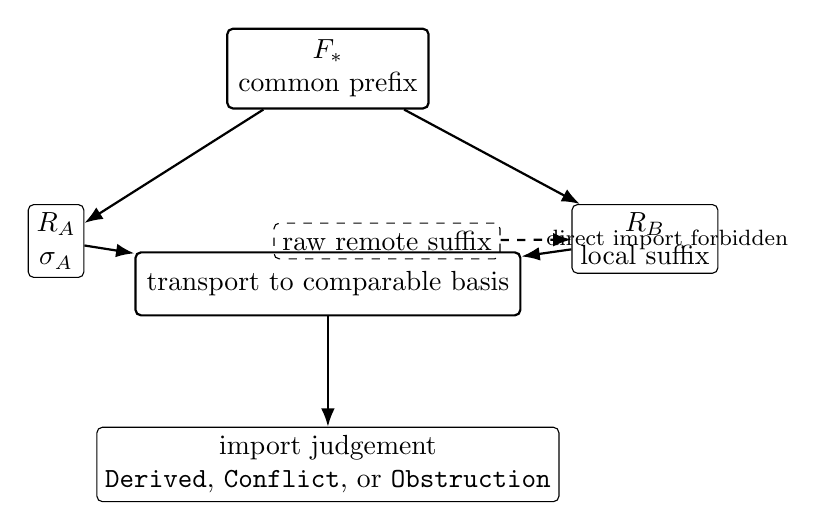
\begin{tikzpicture}[node distance=12mm and 18mm]
  \node[warpbox] (prefix) {\(F_*\)\\common prefix};
  \node[warpsmall, below left=of prefix] (ra) {\(R_A\)\\\(\sigma_A\)};
  \node[warpsmall, below right=of prefix] (rb) {\(R_B\)\\local suffix};
  \node[warpghost, right=24mm of ra] (raw) {raw remote suffix};
  \node[warpbox, below=18mm of prefix] (transport) {transport to comparable basis};
  \node[warpsmall, below=14mm of transport] (import) {import judgement\\\(\texttt{Derived}\), \(\texttt{Conflict}\), or \(\texttt{Obstruction}\)};

  \draw[warparrow] (prefix) -- (ra);
  \draw[warparrow] (prefix) -- (rb);
  \draw[warpblocked] (raw) -- node[warplabel, right] {direct import forbidden} (rb);
  \draw[warparrow] (ra) -- (transport);
  \draw[warparrow] (rb) -- (transport);
  \draw[warparrow] (transport) -- (import);
\end{tikzpicture}

\smallskip
\emph{Figure 3.} A remote suffix cannot be judged directly at the receiver's tip; it must first be transported to a comparable basis.
\end{center}

Admission is impossible until transport has first normalised the remote suffix to a comparable frontier. If that normalisation succeeds, \(\operatorname{Admit}_{\Pi}(F_*, C, \chi)\) can judge the imported claim; if it fails, the result is conflict or obstruction rather than silent patch application. The engineering implication is that replication becomes queryable and auditable as lawful transport, rather than as heuristic packet replay.

\[
\begin{aligned}
\widetilde{C}
&=
\operatorname{Transport}(F_*, \sigma_A, F_B),\\
(R, W)
&=
\operatorname{Admit}_{\Pi}(F_*, \widetilde{C}, \chi),\\
R
&\in
\{\operatorname{Derived}(x), \operatorname{Conflict}, \operatorname{Obstruction}\}.
\end{aligned}
\]

\section{Continuum and the Post-Unix Horizon}

The post-Unix claim of the paper is not that the operating system becomes graph-shaped. It is that the operating system becomes frontier-relative. The intended lineage is Unix's process/file discipline, capability systems' authority discipline, Plan 9's namespace discipline, and EROS-style capability persistence; \WARP{} shifts the centre of gravity from container, descriptor, or address space to witnessed causal admission over shared history \cite{ritchie1974unix,dennis1966programming,pike1995plan9,shapiro1999eros}.

An inadequate formulation is:

\begin{quote}
process = divergent worldline
\end{quote}

The formulation we require is:

\begin{quote}
process = strand whose live realisation is a shadow working set over shared machine history
\end{quote}

This changes the meaning of ownership, isolation, deletion, debugging, and restart. Safety is no longer a byproduct of process opacity. It becomes a property of lawful admission over semantically closed sites. Once that sentence is accepted, the privacy problem becomes explicit: if shared history is primary, the system must still provide a protected interval in which exploratory work does not immediately become collaborative fact.

\paragraph{Application boundary.}
The same post-Unix shift also changes how applications should meet the runtime.
The relevant question is no longer how to add handwritten app methods to a host.
It is how to compile app-authored optic surfaces into lawful set-side intents
and lawful get-side observer plans over one generic holographic runtime. In
that arrangement, the application authors its own nouns, result families, and
reading families; a compiler lowers those surfaces into intent envelopes,
observer plans, and shared codecs; and the runtime remains generic, admitting
intents, emitting outcome/receipt/hologram boundaries, and later serving
bounded readings through hosted observers. Paper VII does not formalise that
compiler boundary, but the architecture developed here makes it the correct
engineering seam rather than a separate theory.

\subsection{The Three-Tier Thinking Room}

Continuum remains socially viable only if retention and revelation are decoupled. We therefore distinguish a three-tier ``thinking room'':

\begin{enumerate}[leftmargin=*]
  \item \textbf{Ephemeral Scratch}: local, weakly retained, and disposable.
  \item \textbf{Author-Only Speculative Lane}: durable, replayable, sealed to the author by default.
  \item \textbf{Shared / Admitted Lane}: collaboratively admitted causal truth.
\end{enumerate}

This is the privacy-preserving answer to post-Unix claustrophobia. The system may remember drafts, but it need not reveal them by default, and it need not retain them indefinitely. Architecturally, Ephemeral Scratch is best understood as pre-admission or minimally retained local work; Author-Only lanes are admitted enough to be durable and replayable without yet being socially transported; Shared lanes mark the moment private speculation crosses into collaborative truth.

This distinction matters immediately for debugger-driven counterfactual work. A reading, replay, or inspection act does not by itself create new causal truth; it is revelation only. If an operator explicitly asks to continue from an earlier coordinate or explore a counterfactual alternative, the system should emit an explicit fork rooted at an exact fork basis. Such debugger-created strands are real causal objects, but they should default to Ephemeral Scratch or an Author-Only Speculative Lane rather than crossing directly into shared history. When retained, their provenance should record the creating principal, tool or session origin, fork basis, and retention or revelation posture. Only an explicit promotion should move them into the Shared / Admitted Lane.

\section{Privacy, Provenance, and Revelation}

Paper VI argued that privacy and provenance are not mutually exclusive. Paper VII's job is to show the architecture that makes that coexistence credible. Three components matter here.

\subsection{Property Library}

Private speculative lanes should not need to expose their interior autobiography in order to collaborate. This is where provenance meets information-flow control and zero-knowledge style selective evidence \cite{denning1976lattice,myers1999jflow,goldwasser1989knowledge}. Instead, they should emit a certificate of lawfulness: property-bearing evidence that type/resource safety, admission integrity, provenance linkage, and policy conformance hold at the required tier. Concretely, such a certificate should minimally identify the shared basis to which it refers, the property set it attests, the witness or proof tier under which those properties were established, and the shell anchors needed for later replay, audit, or revocation. In that sense the certificate is a special case of the generic package \(\theta\): not the witness itself, but a carrier of witness-bearing consequences upon which others may lawfully rely. Some of these properties may survive fold-to-opaque as shell anchors or zero-knowledge proofs; others, such as full forensic traces, require later unsealing.

\subsection{Reliance Status}

Once certificates exist, trust itself becomes a first-class object with a lifecycle, echoing the lifecycle pressure visible in PKI and certificate revocation systems while generalising the object being trusted \cite{rfc5280}. A certificate can be issued, activated, superseded, suspended, revoked, expired, and archived. Revocation is not deletion. It is a new witnessed status transition about future lawful reliance. This creates a true reliance domain within \WARP{}, rather than leaving trust as an external social assumption.

\subsection{Observer Rights}

The subject-side counterpart is an observer rights lattice governing who may discover, inspect, rely on, unseal, replay, export, delegate, or revoke access over proof-bearing artefacts. On this side of the architecture, the right local noun is not ``lens'' but ``reading'': an observer, equipped with a bounded reading frame, obtains a lawful projection by decoding only the least required slice of a subject's backward causal cone. In the stronger ontology above, that reading is a coordinate chart over causal history rather than a glimpse of a privileged graph-in-itself. Different observers may therefore lawfully emit different charts over the same history, and revelation law must govern which transitions between such charts are permitted, what witness must travel with them, and what plurality or obstruction must remain explicit. This is where the architecture meets Paper VI's observer classes, replay impact labels, and bounded warrants. High-impact revelation rights should be understood as activated rather than ambient, often requiring threshold or role-separated co-authorisation.

\section{Open Frontier Questions}

The architectural centre is now sufficiently stable for the remaining work to be treated as extension rather than rescue. The next frontier laws likely include:

\begin{itemize}[leftmargin=*]
  \item \textbf{exposure ledger and contamination calculus},
  \item collective sovereignty over co-owned traces,
  \item mode-transition contamination and stale certificate handling,
  \item \textbf{revocation propagation over dependency graphs},
  \item lawful compilation of app-authored optics into intent and observer plans,
  \item export semantics at the substrate boundary,
  \item aperture decay as a witnessed act,
  \item temporal-logic query languages over lawful transport, admission, and revelation paths.
\end{itemize}

These are not signs that the foundations are incomplete. They are what becomes visible once the foundations are coherent enough to support a real social-runtime theory. The first two pressure points for the next paper are the exposure ledger and contamination calculus, followed by revocation propagation, because both are prerequisites for any serious account of collective sovereignty or long-range social debugging.

\section{Conclusion}

The central result of this paper is not a single algorithm. It is a reframing. \WARP{} is a system in which existence is autobiographical and collaboration is the witnessed admission of mutual reliance. State transitions, braid outcomes, certificate trust, historical folding, and observer revelation all become instances of the same deeper architectural law.

That law does not eliminate judgement, wisdom, or subjectivity. Observers remain outside the algebra in the decisive sense: the system can govern what is revealed and why it is trustworthy, but it cannot force a reader to find a derivation elegant, persuasive, or humane. What it can do is make the terms of collaboration explicit. In a \WARP{}-native world, software does not merely execute. It commits, folds, and reveals truth under law.


\begin{thebibliography}{99}

\bibitem{lamport1978time}
Leslie Lamport.
\newblock Time, clocks, and the ordering of events in a distributed system.
\newblock \textit{Communications of the ACM}, 21(7):558--565, 1978.

\bibitem{winskel1986event}
Glynn Winskel.
\newblock Event structures.
\newblock In \textit{Advances in Petri Nets 1986}, Lecture Notes in Computer Science 255, pages 325--392. Springer, 1987.

\bibitem{ehrig1973graph}
Hartmut Ehrig, Michael Pfender, and Hans Jürgen Schneider.
\newblock Graph-grammars: an algebraic approach.
\newblock In \textit{Proceedings of the 14th Annual Symposium on Switching and Automata Theory}, pages 167--180. IEEE, 1973.

\bibitem{corradini1997algebraic}
Andrea Corradini, Hartmut Ehrig, Michael Löwe, Ugo Montanari, and Francesca Rossi.
\newblock Algebraic approaches to graph transformation, Part I: basic concepts and double pushout approach.
\newblock In Grzegorz Rozenberg, editor, \textit{Handbook of Graph Grammars and Computing by Graph Transformation}, Volume 1. World Scientific, 1997.

\bibitem{weiser1981program}
Mark Weiser.
\newblock Program slicing.
\newblock In \textit{Proceedings of the 5th International Conference on Software Engineering}, pages 439--449. IEEE Computer Society, 1981.

\bibitem{buneman2001why}
Peter Buneman, Sanjeev Khanna, and Wang-Chiew Tan.
\newblock Why and where: a characterization of data provenance.
\newblock In \textit{Proceedings of the International Conference on Database Theory}, pages 316--330. Springer, 2001.

\bibitem{green2007provenance}
Todd J. Green, Grigoris Karvounarakis, and Val Tannen.
\newblock Provenance semirings.
\newblock In \textit{Proceedings of the ACM Symposium on Principles of Database Systems}, pages 31--40. ACM, 2007.

\bibitem{cheney2009provenance}
James Cheney, Laura Chiticariu, and Wang-Chiew Tan.
\newblock Provenance in databases: why, how, and where.
\newblock \textit{Foundations and Trends in Databases}, 1(4):379--474, 2009.

\bibitem{jacobson2009darcs}
Judah Jacobson.
\newblock A formalization of Darcs patch theory using inverse semigroups.
\newblock \textit{arXiv:0911.2852}, 2009.

\bibitem{mimram2013patch}
Samuel Mimram and Cinzia Di Giusto.
\newblock A categorical theory of patches.
\newblock \textit{Electronic Proceedings in Theoretical Computer Science}, 138:283--307, 2013.

\bibitem{fowler2005eventsourcing}
Martin Fowler.
\newblock Event sourcing.
\newblock martinfowler.com, 2005.

\bibitem{decandia2007dynamo}
Giuseppe DeCandia, Deniz Hastorun, Madan Jampani, Gunavardhan Kakulapati, Avinash Lakshman, Alex Pilchin, Swaminathan Sivasubramanian, Peter Vosshall, and Werner Vogels.
\newblock Dynamo: Amazon's highly available key-value store.
\newblock In \textit{Proceedings of the ACM Symposium on Operating Systems Principles}, pages 205--220. ACM, 2007.

\bibitem{shapiro2011crdt}
Marc Shapiro, Nuno Preguiça, Carlos Baquero, and Marek Zawirski.
\newblock A comprehensive study of convergent and commutative replicated data types.
\newblock INRIA Research Report RR-7506, 2011.

\bibitem{ellis1989groupware}
Clarence A. Ellis and Simon J. Gibbs.
\newblock Concurrency control in groupware systems.
\newblock In \textit{Proceedings of the ACM SIGMOD International Conference on Management of Data}, pages 399--407. ACM, 1989.

\bibitem{park1981concurrency}
David Park.
\newblock Concurrency and automata on infinite sequences.
\newblock In \textit{Theoretical Computer Science}, Lecture Notes in Computer Science 104, pages 167--183. Springer, 1981.

\bibitem{milner1989communication}
Robin Milner.
\newblock \textit{Communication and Concurrency}.
\newblock Prentice Hall, 1989.

\bibitem{martinlof1984intuitionistic}
Per Martin-Löf.
\newblock \textit{Intuitionistic Type Theory}.
\newblock Bibliopolis, 1984.

\bibitem{ritchie1974unix}
Dennis M. Ritchie and Ken Thompson.
\newblock The UNIX time-sharing system.
\newblock \textit{Communications of the ACM}, 17(7):365--375, 1974.

\bibitem{dennis1966programming}
Jack B. Dennis and Earl C. Van Horn.
\newblock Programming semantics for multiprogrammed computations.
\newblock \textit{Communications of the ACM}, 9(3):143--155, 1966.

\bibitem{pike1995plan9}
Rob Pike, Dave Presotto, Sean Dorward, Bob Flandrena, Ken Thompson, Howard Trickey, and Phil Winterbottom.
\newblock Plan 9 from Bell Labs.
\newblock \textit{Computing Systems}, 8(3):221--254, 1995.

\bibitem{shapiro1999eros}
Jonathan S. Shapiro, Jonathan M. Smith, and David J. Farber.
\newblock EROS: a fast capability system.
\newblock In \textit{Proceedings of the ACM Symposium on Operating Systems Principles}, pages 170--185. ACM, 1999.

\bibitem{denning1976lattice}
Dorothy E. Denning.
\newblock A lattice model of secure information flow.
\newblock \textit{Communications of the ACM}, 19(5):236--243, 1976.

\bibitem{myers1999jflow}
Andrew C. Myers.
\newblock JFlow: practical mostly-static information flow control.
\newblock In \textit{Proceedings of the ACM Symposium on Principles of Programming Languages}, pages 228--241. ACM, 1999.

\bibitem{goldwasser1989knowledge}
Shafi Goldwasser, Silvio Micali, and Charles Rackoff.
\newblock The knowledge complexity of interactive proof systems.
\newblock \textit{SIAM Journal on Computing}, 18(1):186--208, 1989.

\bibitem{rfc5280}
David Cooper, Stefan Santesson, Stephen Farrell, Sharon Boeyen, Russell Housley, and William Polk.
\newblock Internet X.509 Public Key Infrastructure Certificate and Certificate Revocation List (CRL) Profile.
\newblock RFC 5280, 2008.

\end{thebibliography}

\end{document}
